% --- SLIDE 7: Beyond Bits: General Alphabets ---
\begin{frame}{Beyond Bitvectors: General Alphabets}
    \framesubtitle{Wavelet Trees}
    \vspace{-0.2em}
    What about sequences $S[1..n]$ over larger alphabets $\Sigma = \{1, \dots, \sigma\}$?
    \begin{figure}[hbtp]
        \centering
        \only<2>{
\includegraphics[width=0.6\textwidth]{assets/wt1.pdf}} % Visible only on slide 2
        \only<3>{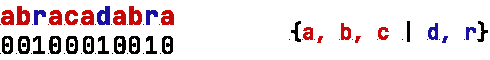
\includegraphics[width=0.7\textwidth]{assets/wt2.pdf}} % Visible only on slide 3
        \only<4>{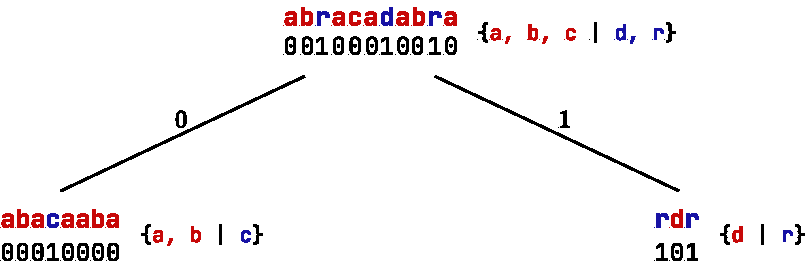
\includegraphics[width=\textwidth]{assets/wt3.pdf}} % Visible only on slide 4
        \only<5>{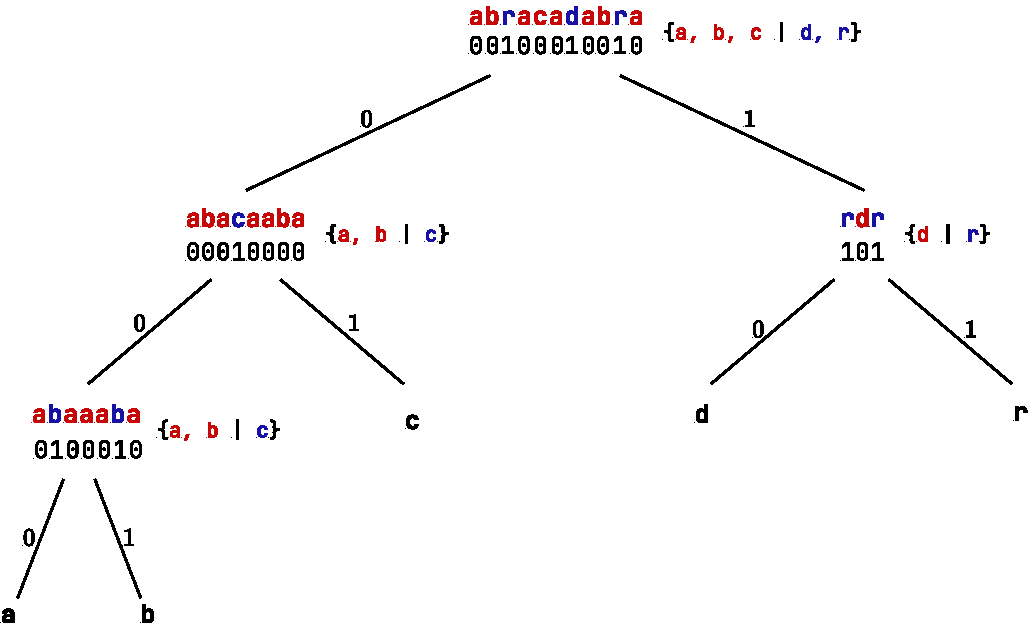
\includegraphics[width=0.7\textwidth]{assets/wt4.pdf}} % Visible ONLY on slide 5
    \end{figure}
    \only<6->{
        \begin{columns}[T] % Align columns at the top
            \begin{column}{0.55\textwidth} % Adjust width as needed
                \centering % Center the image in the column
                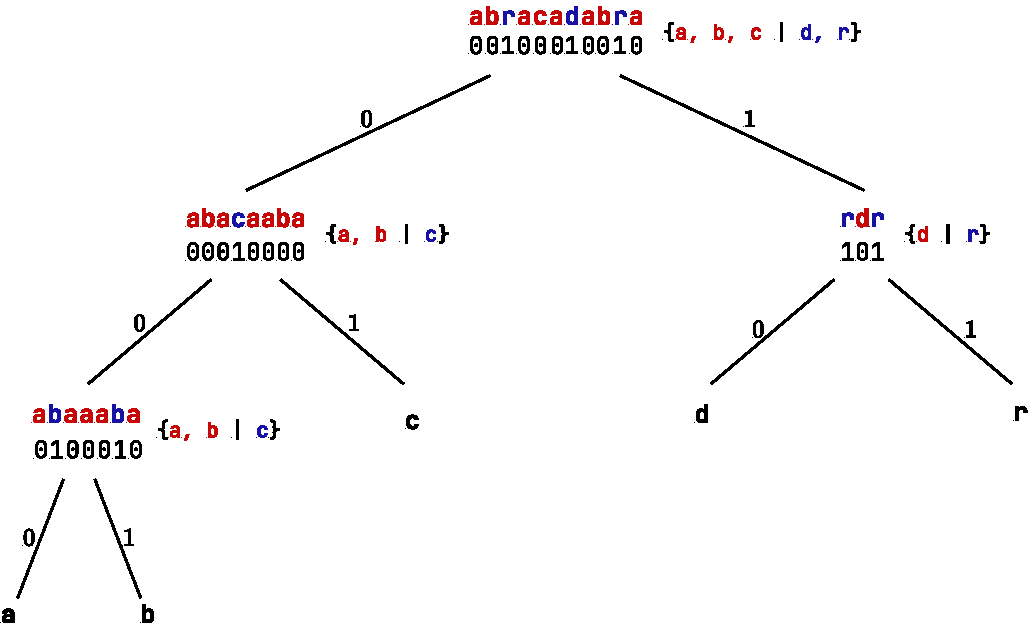
\includegraphics[width=\textwidth]{assets/wt4.pdf} % Show from slide 6 onwards
            \end{column}
            \begin{column}{0.45\textwidth} % Adjust width as needed
                \begin{block}{$\mathcal{H}_0$-Compressed Wavelet Tree} % Ref Thm 3.8 in thesis
                    Using RRR for bitvectors:
                    \begin{itemize}
                        \item \textbf{Space}: $n \mathcal{H}_0(S) + o(n \log \sigma)$ bits.
                        \item \textbf{Query Time}: $O(\log \sigma)$ for \textsf{access}, \textsf{rank}$_c$, \textsf{select}$_c$.
                    \end{itemize}
                    Adapts space to the sequence's zero-order entropy.
                \end{block}
            \end{column}
        \end{columns}
    }
\end{frame}

% \begin{frame}{Wavelet Tree Construction: Example}
%     \framesubtitle{Step 1: Splitting the Root}
%     \begin{columns}[T,totalwidth=\textwidth] % Colonne allineate in alto
%         % Colonna sinistra: Spiegazioni
%         \begin{column}{0.5\textwidth}
%             % Spazio sopra allineato con l'alfabeto a destra
%             \vspace*{1ex} % Aggiusta se necessario

%             \uncover<1->{
%                 \textbf{1. Alphabet Split:}
%                 \begin{itemize}
%                     \item Root covers $\Sigma = \{\texttt{a, b, c, d, r}\}$.
%                     \item Use range $[1, 5]$.
%                     \item Midpoint $m = 3$ is \alert{c}.
%                     \item Split into: $[\texttt{a, b, c}]$ vs $[\texttt{d, r}]$.
%                 \end{itemize}
%                 \bigskip
%             }
%             \uncover<2->{
%                 \textbf{2. Bitmap Rule ($B_{root}$):}
%                 \begin{itemize}
%                     \item If char $\le$ \alert{c} $\rightarrow$ Bit \textcolor{blue!70!black}{0} (Goes Left)
%                     \item If char $>$ \alert{c} $\rightarrow$ Bit \textcolor{red!70!black}{1} (Goes Right)
%                 \end{itemize}
%                 \bigskip
%             }
%         \end{column}

%         % Colonna destra: Visualizzazione
%         \begin{column}{0.5\textwidth}
%             \centering
%             % Spazio sopra allineato con l'alfabeto a sinistra
%             \vspace*{9ex} % Aggiusta se necessario

%             % Visualizzazione dell'alfabeto
%             \uncover<2->{
\includegraphics[width=0.5\textwidth]{../bachelor-thesis/TeX/assets/WT_slides_root.pdf}} % Mostra solo quando necessario
%         \end{column}
%     \end{columns}
% \end{frame}

% \begin{frame}{Wavelet Tree Construction: Example}
%     \framesubtitle{Building the Tree}
%     \begin{figure}[hbtp]
%         \centering
%         % Replace TikZ with sequential images
%         \only<1>{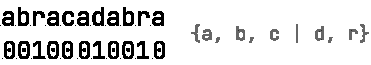
\includegraphics[width=0.7\textwidth]{../bachelor-thesis/TeX/assets/WT_slides1.pdf}} % Visible only on slide 2
%         \only<2>{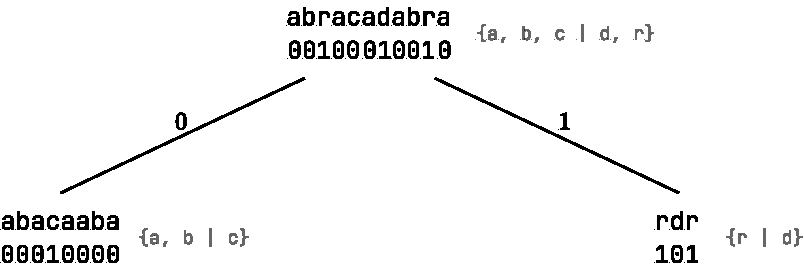
\includegraphics[width=0.7\textwidth]{../bachelor-thesis/TeX/assets/WT_slides2.pdf}} % Visible only on slide 3
%         \only<3->{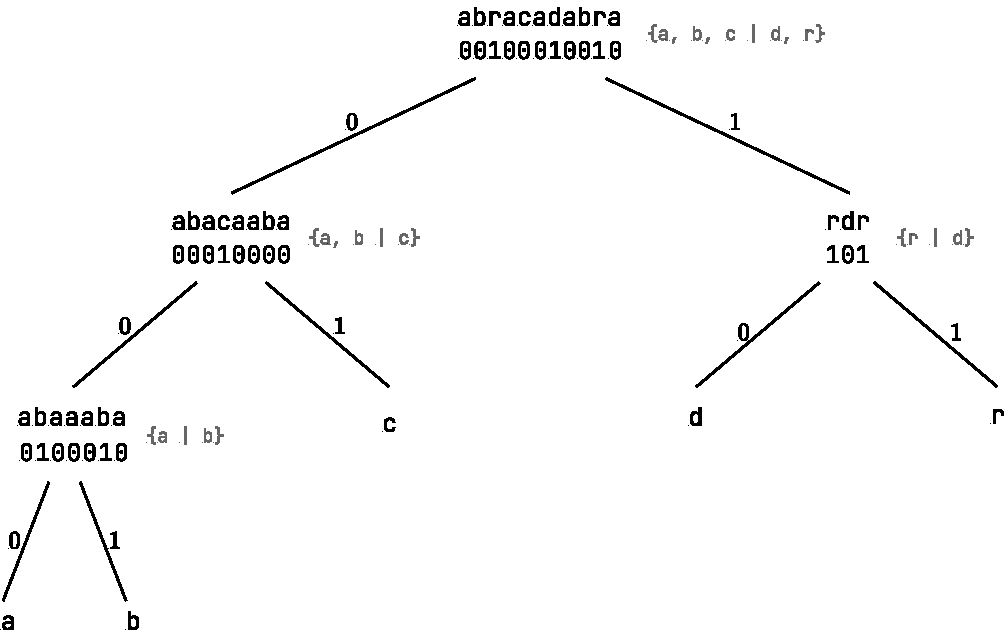
\includegraphics[width=0.7\textwidth]{../bachelor-thesis/TeX/assets/WT_slides3.pdf}} % Visible from slide 4 onwards
%         % \caption{Hierarchical structure for Rank}
%     \end{figure}
% \end{frame}

% \begin{frame}{Wavelet Tree: Rank Example}
%     \framesubtitle{Rank on Wavelet Trees}

%     \begin{figure}[hbtp]
%         \centering
%         % Replace TikZ with sequential images
%         \only<1>{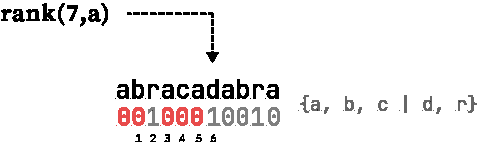
\includegraphics[width=0.7\textwidth]{../bachelor-thesis/TeX/assets/WT_rank_slides1.pdf}} % Visible only on slide 2
%         \only<2>{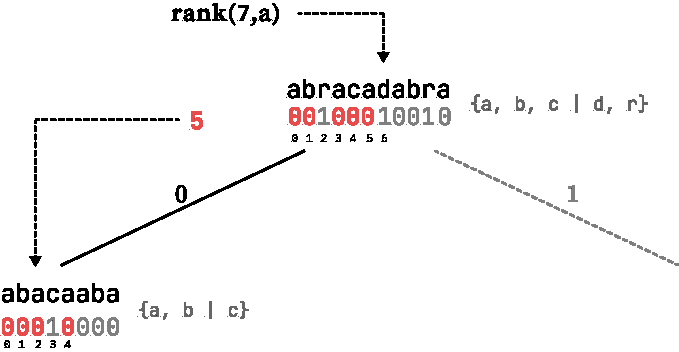
\includegraphics[width=0.7\textwidth]{../bachelor-thesis/TeX/assets/WT_rank_slides2.pdf}} % Visible only on slide 3
%         \only<3->{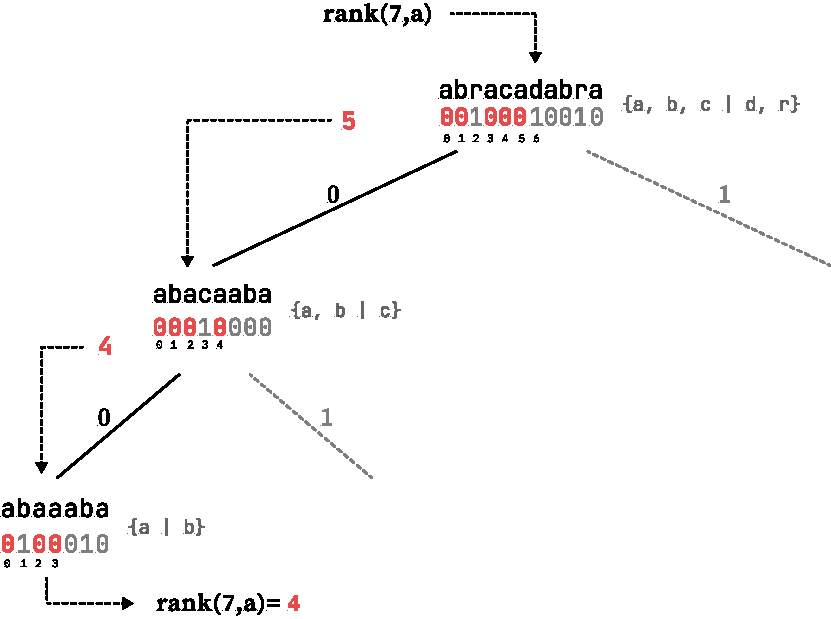
\includegraphics[width=0.65\textwidth]{../bachelor-thesis/TeX/assets/WT_rank_slides3.pdf}} % Visible from slide 4 onwards
%         % \caption{Hierarchical structure for Rank}
%     \end{figure}
% \end{frame}

% % --- SLIDE 8: Wavelet Tree Performance Summary ---
% \begin{frame}{Wavelet Tree: Performance Summary}
%     \framesubtitle{Space and Query Time}

%     % Standard WT Result
%     \begin{theorem}[Standard Wavelet Tree]
%         Represents $S[1..n]$ over $\Sigma=\{1,\dots,\sigma\}$ using:
%         \begin{itemize}
%             \item \textbf{Space}: $n \lceil \log \sigma \rceil + o(n \log \sigma)$ bits.
%             \item \textbf{Query Time}: $O(\log \sigma)$ for \textsf{access}, \textsf{rank}$_c$, \textsf{select}$_c$.
%         \end{itemize}
%     \end{theorem}

%     \pause % Introduce compressed versions

%     % Compressed WT (H0)
%     \begin{theorem}[$\mathcal{H}_0$-Compressed Wavelet Tree] % Ref Thm 3.8 in thesis
%         Using RRR for bitvectors:
%         \begin{itemize}
%             \item \textbf{Space}: $n \mathcal{H}_0(S) + o(n \log \sigma)$ bits.
%             \item \textbf{Query Time}: $O(\log \sigma)$ for \textsf{access}, \textsf{rank}$_c$, \textsf{select}$_c$.
%         \end{itemize}
%         Adapts space to the sequence's zero-order entropy.
%     \end{theorem}
% \end{frame}
